%+*** mainfile.tex
% arara: pdflatex: { files: [ mainfile.tex ] }
% !arara: indent: { overwrite: on, trace: yes, localSettings: on}
\chapter{The quadratic formula and functions}
\minitoc
\section{The Quadratic Formula}
\textref{10.3}{614}%
We have so far solved some \gls{quadratic} equations by factoring, and using the square root property. There
are two other options: completing the square (which you will discuss in Math 95), and the quadratic
formula, which is the focus of this section.

\begin{myDefinition}
	Given a quadratic \gls{equation}
	\[
		ax^2 + bx + c = 0 \qquad (a\ne 0)
	\]
	then it can be shown that the two solutions are
	\[
		x = \frac{-b+\sqrt{b^2-4ac}}{2a} \qquad or \qquad x = \frac{-b-\sqrt{b^2-4ac}}{2a}
	\]
	These solutions can be written more efficiently as
	\[
		x = \frac{-b\pm \sqrt{b^2-4ac}}{2a}
	\]
	This is known as the {\em quadratic formula.}
\end{myDefinition} 

There will be at most two real solutions to a quadratic equation, and the quadratic formula will work for {\em any} quadratic
equation. We will demonstrate how to use it in this section, and give examples that have two real solutions, one real \gls{solution}, 
and no real solutions.

\begin{myexample}
\Gls{solve}
\[
	2x^2+9x-5=0
\]
using the quadratic formula.
\end{myexample}
\begin{myProof}
	We begin by identifying the coefficients $a$, $b$, and $c$. This is easily done by remembering that $a$ is
	the \gls{coefficient} of the $x^2$ term, $b$ is the coefficient of the $x$ term, and $c$ is the constant coefficient. 
	Therefore, in this example
	\[
		a = 2, \qquad b=9, \qquad c = -5
	\]
	Remember that $a$, $b$, and $c$ will always be {\em numbers}, and we are trying to find values of $x$ that satisfy the 
	given equation.
				
	Note that the directions ask us to solve the equation using the quadratic formula- it may help you to write out the 
	quadratic formula before starting each problem, and it is well worth memorizing for this class, and for all future Math classes. Take care
	to extend the fraction bar the entire length of the numerator
	\begin{align*}
		x & =  \frac{-b\pm \sqrt{b^2-4ac}}{2a}                                     \\
		  & =  \frac{-9\pm\sqrt{9^2-4(2)(-5)}}{2(2)}                               \\
		  & =  \frac{-9\pm \sqrt{81-(-40)}}{4}                                     \\
		  & =  \frac{-9\pm\sqrt{121}}{4}                                           \\
		  & =  \frac{-9+11}{4} = \frac{1}{2} \qquad or\qquad  \frac{-9-11}{4} = -5 
	\end{align*} 
	The solution set to the given quadratic equation is
	\[
		\left\{\frac{1}{2}, -5\right\}
	\]
	The check is left as an exercise.
				
	Notice in this example that the problem can also be solved by factoring
	\[
		(2x-1)(x+5)=0
	\]
	which gives the solution set
	\[
		\left\{\frac{1}{2}, -5\right\}
	\]
	as before.
\end{myProof} 

\begin{myexample}\label{ex:quadform1}
Solve the following quadratic equation
\[
	x^2=9 
\]
using the quadratic formula.
\end{myexample}
\begin{myProof}
	Note that we could solve this equation by factoring, or by using the square root property, however
	the problem asks us to use the quadratic formula. In order to do so we first need to set the equation
	equal to 0, which we do by subtracting 9 from both sides
	\[
		x^2-9 = 0
	\]
				
	We now need to identify the values of $a$, $b$, and $c$; in our example we see that
	\[
		a = 1, \qquad b=0, \qquad c = -9
	\] 
	Following along the same lines as in the previous example, we have
	\begin{align*}
		x & =  \frac{-b\pm \sqrt{b^2-4ac}}{2a}       \\
		  & =  \frac{-0\pm\sqrt{0^2-4(1)(-9)}}{2(1)} \\
		  & =  \frac{0\pm\sqrt{36}}{2}               \\
		  & = \pm\frac{6}{2}                         \\
		  & = \pm 3                                  
	\end{align*} 
	The solution set to the equation is
	\[
		{-3,3}
	\]
	As in the previous example, you should check these solutions in the original equation (one at a time). 
				
	Note that if you had solved this problem by factoring, then the first step would have been to write
	\[
		(x-3)(x+3)=0
	\]
	from which it follows that the solution set is as before.
				
\end{myProof} 
\begin{myDefinition}
	When using the square root property or the quadratic formula, do not forget that
	there are two solutions because of the $\pm$ sign.
\end{myDefinition} 

\begin{myexample}
Solve
\[
	x^2+2x+1=0
\]
using the quadratic formula.
\end{myexample}
\begin{myProof}
	Note that we have so far encountered only examples that have two real solutions. This example gives a slightly
	different result
	\begin{align*}
		x & =  \frac{-b\pm \sqrt{b^2-4ac}}{2a}      \\
		  & =  \frac{-2\pm\sqrt{2^2-4(1)(1)}}{2(1)} \\
		  & =  \frac{-2\pm\sqrt{0}}{2}              \\
		  & =  -1                                   
	\end{align*}
	This example is interesting, as we have only {\em one real solution}. In this case, we say that we have one real
	repeated solution.
				
	Note that if you had solved the equation by factoring the first step would have been to write the equation as
	\[
		(x+1)^2=0
	\]
	from which it follows that $x=-1$ twice, as before.
\end{myProof} 

\begin{myexample}
Solve
\[
	x^2=x+6
\]
using the quadratic formula.
\end{myexample}
\begin{myProof}
	We begin by setting the equation equal to 0,
	\[
		x^2-x-6=0
	\]
	which allows us to identify that
	\[
		a = 1, \qquad b = -1, \qquad c = -6
	\]
	We proceed as in the previous examples
	\begin{align*}
		x & =  \frac{-b\pm \sqrt{b^2-4ac}}{2a}        \\
		  & =  \frac{1\pm\sqrt{(-1)^2-4(1)(6)}}{2(1)} \\
		  & =  \frac{1\pm \sqrt{1-24}}{2}             \\
		  & =  \frac{1\pm\sqrt{-23}}{2}               
	\end{align*}
	{}
	Notice here that we have ended with an \gls{expression} containing the square root of a negative number. 
	The result of taking the square root of a negative number is {\em not } real; in this case, 
	we therefore say that the equation has {\em no real solutions}.
\end{myProof} 

\section{Relations and functions}
\textref{10.6}{642}%
The concept of {\em relations} and {\em functions} is fundamental to mathematics. In fact, we have
been dealing with functions throughout the class so far, it's just that we have not referred to them as this.
\begin{itemize}
	\item A {\em relation} is a rule or set of rules that maps an element in the 
	domain to an element in the range.
	\item A {\em function} is a relation that maps an element in the domain onto 
	a single element in the range.
\end{itemize} 

\begin{center}
	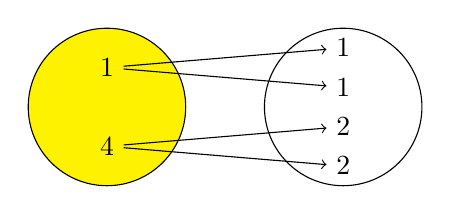
\begin{tikzpicture}
		\filldraw [yellow,draw=black] (0,0) circle (1) node (mydomain){};
		\node (d1) at (0,.5) {$1$};
		\node (d2) at (0,-.5){$4$};
		\draw  (3,0) circle (1);
		\node (r1) at (3,.75) {$1$};
		\node (r2) at (3,.25){$1$};
		\node (r3) at (3,-.25){$2$};
		\node (r4) at (3,-.75){$2$};
		\draw[->] (d1)--(r1);
		\draw[->] (d1)--(r2);
		\draw[->] (d2)--(r3);
		\draw[->] (d2)--(r4);
	\end{tikzpicture}
	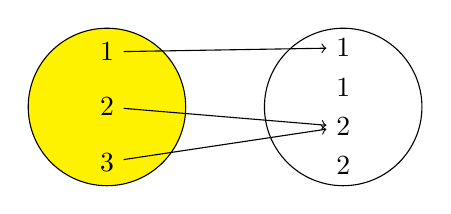
\begin{tikzpicture}
		\filldraw [yellow,draw=black] (0,0) circle (1) node (mydomain){};
		\node (d1) at (0,.7) {$1$};
		\node (d2) at (0,0){$2$};
		\node (d3) at (0,-.7){$3$};
		\draw  (3,0) circle (1);
		\node (r1) at (3,.75) {$1$};
		\node (r2) at (3,.25){$1$};
		\node (r3) at (3,-.25){$2$};
		\node (r4) at (3,-.75){$2$};
		\draw[->] (d1)--(r1);
		\draw[->] (d2)--(r3);
		\draw[->] (d3)--(r3);
	\end{tikzpicture}
\end{center}

\begin{itemize}
	\item The domain of a function is the {\em input} set. In the above, the domain of the function $F$ is $\{1,2,3\}$.
	\item The range of a function is the {\em output} set. In the above, the range of the function $F$ is $\{1,-1,2,2\}$.
\end{itemize} 
Notice the distinction between a {\em relation} and a {\em function}. A function takes each element from the input set and
maps it into only one element in the output set- the relation $N$ is not a function as the number 1 goes to both 1 and -1 (notice
also that 4 goes to 2 and -2).

\subsection{Function notation}
We represent a function algebraically using the notation $f(x)$. For example, we can define the \gls{linear} function
\[
	f(x)=2x+3
\]
\begin{itemize}
	\item we pronounce $f(x)$ as `$f$ of $x$', and say that $f$ is a function of $x$
	\item $x$ is the input \gls{variable}, or more commonly known as the {\em independent variable}
\end{itemize} 
Let's say that we want to evaluate this function at $x=4$. To do this we write
\begin{align*}
	f(4) & =		2(4)-3 \\
	     & =		8-3    \\
	     & =		5      
\end{align*} 
Notice that we write the \gls{point} that we want to evaluate in the parenthesis on the left hand side, 
and replace each occurrence of $x$ with 4 on the right hand side.

We may also write $y=2x-3$, in which case we still say that $x$ is the independent variable, 
and that $y$ is the {\em dependent} variable. 

\begin{myexample}
Let $f$ be the function that has formula
\[
	f(x)=x^2+2
\]
Evaluate 
\begin{multicols}{3}
	\begin{enumerate}
		\item $f(2)$
		\item $f(0)$
		\item $f(-4)$
	\end{enumerate} 
\end{multicols}
\end{myexample}
\begin{myProof}
	\begin{enumerate}
		\item 
		$\begin{aligned}[t]
			f(2) & =		2^2+2 \\
			     & =		4+2   \\
			     & =		6     
		\end{aligned}$
		\item 
		$\begin{aligned}[t]
			f(0) & =		0^2+2 \\
			     & =		0+2   \\
			     & =		2     
		\end{aligned}$
		\item 
		$\begin{aligned}[t]
			f(-4) & =		(-4)^2+2 \\
			      & =		16+2     \\
			      & =		18       
		\end{aligned}$
	\end{enumerate} 
\end{myProof} 

\begin{myexample}
\drillandskill
Let
\[
	f(x) = 4x-3
\]
Find each of the following
\begin{multicols}{4}
	\begin{enumerate}
		\item $f(2)$ \solution{$=5$}
		\item $f(0)$\solution{$=-3$}
		\item $f(1)$\solution{$=1$}
		\item $f(3)$\solution{$=9$}
	\end{enumerate}
\end{multicols}
\end{myexample}

\begin{myexample}
\drillandskill
Let $g$ be the function that has formula
\[
	g(x) = x^2 + 2x +3 
\]
Find each of the following
\begin{multicols}{4}
	\begin{enumerate}
		\item $g(2)$\solution{$=11$}
		\item $g(0)$\solution{$=3$}
		\item $g(1)$\solution{$=6$}
		\item $g(3)$\solution{$=18$}
	\end{enumerate}
\end{multicols}
\end{myexample}

\begin{myexample}
Let's interpret each of the following functions verbally
\begin{description}
	\item $y=x+2$      $y$ is equal to $x$ plus 2          	
	\item $f(x)=x+2$   $f$ of $x$ is equal to $x$ plus 2   
	\item $u=3t-5$     $u$ is equal to $3t$ minus 5        
	\item $g(t)=3t-5$  $g$ of $t$ is equal to $3t$ minus 5 
\end{description}
\end{myexample}

\begin{myexample}
The law firm of BDD charges an account set up fee of \$1,000.00 and charges a consultation
rate of \$100.00 per hour. Find $B(t)$, the cost of dealing with this firm as a function of time, $t$
in hours. 

Evaluate $B(1)$, $B(2)$, and $B(3)$.
\end{myexample}
\begin{myProof}
	We recognize that this is an example of a linear function, and we can write
	\[
		B(t)=1000+100t
	\]
	where $t\geq 0$. We evaluate the function by using the above method of replacing the independent
	variable with whatever is in the parenthesis.
	\begin{align*}
		B(1) & =	 1000+100(1) & B(2) & =	 1000+100(2) & B(3) & =	 1000+100(3) \\
		     & =	 1000+100    &      & =	 1000+200    &      & =	 1000+300    \\
		     & =	 1100        &      & =	 1200        &      & =	 1300        
	\end{align*} 
	These represent the cost of setting up an account that takes 1 hour, 2 hours, and 3hours
	respectively.
\end{myProof} 


\begin{myexample}
Let $f$ be the function that has formula
\[
	f(x) = 4x-2
\]
which is shown in \cref{fig:linfunctioneval}. Find the following
\begin{multicols}{3}
	\begin{enumerate}
		\item $f(0)$
		\item $f(1)$
		\item $f(-3)$
	\end{enumerate} 
\end{multicols}
{}
\end{myexample}
\begin{figure}[!h]
	\centering
	\begin{tikzpicture}
		\begin{axis}[
				framed,
				xmin=-10,xmax=10,
				ymin=-10,ymax=10,
				xtick={-8,-6,...,8},
				minor xtick={-9,-7,...,9},
				ytick={-8,-6,...,8},
				minor ytick={-9,-7,...,9},
				grid=both,
			]
			\addplot expression[domain=-2:3,samples=100]{4*x-2};
			\legend{$f(x)=4x-2$};
		\end{axis}
	\end{tikzpicture}
	\caption{$f(x)=4x-2$}
	\label{fig:linfunctioneval}
\end{figure}
\begin{myProof}
	\begin{enumerate}
		\item To find $f(0)$ we are looking for the $y$ value when $x=0$; we go to 0 on the 
		horizontal axis, and then go down (in this case) until we hit the line. We conclude that
		\[
			f(0)=-2
		\]
		\item To find $f(1)$ we are looking for the $y$ value when $x=1$; we go to 1 on the 
		horizontal axis, and then go up (in this case) until we hit the line. We conclude that
		\[
			f(1) = 2
		\]  
		\item To find $f(-3)$ we proceed as in the previous parts of the problem. However, we see immediately
		that we will not be able to use \cref{fig:linfunctioneval}, because the $y$ value corresponding
		to $x=-3$ is not shown. We therefore find $f(-3)$ algebraically as follows
		\begin{align*}
			f(-3) & =  4(-3)-2 \\
			      & =  -12-2   \\
			      & =  -14     
		\end{align*} 
	\end{enumerate} 
	{}
\end{myProof} 
\FloatBarrier

\begin{myexample}\label{ex:quadraticeval}
The function $g$ has formula
\[
	g(x) = 5-x
\]
and is shown in \cref{fig:linfunctionevalfindx}. Find the values of $x$ for which
\begin{multicols}{2}
	\begin{enumerate}
		\item $g(x)=4$
		\item $g(x)=-1$
	\end{enumerate} 
\end{multicols}
{}
\end{myexample}
\begin{figure}[!h]
	\centering
	\begin{tikzpicture}
		\begin{axis}[
				framed,
				xmin=-10,xmax=10,
				ymin=-10,ymax=10,
				xtick={-8,-6,...,8},
				minor xtick={-9,-7,...,9},
				ytick={-8,-6,...,8},
				minor ytick={-9,-7,...,9},
				grid=both,
			]
			\addplot expression[domain=-5:10,samples=100]{5-x};
			\legend{$g(x)=5-x$};
		\end{axis}
	\end{tikzpicture}
	\caption{$g(x)=5-x$}
	\label{fig:linfunctionevalfindx}
\end{figure}
\begin{myProof}
	\begin{enumerate}
		\item We want to find the value of $x$ for which $g(x)=4$. We are given the $y$ value, and need to find the $x$ value, so we 
		proceed by going to 4 on the $y$ axis, and then go horizontally until we hit the line- we then go down (in this case) until
		we hit the horizontal axis. This gives that
		\[
			g(1)=4
		\]
		An alternative approach to this problem is to solve the equation
		\[
			4 = 5-x
		\]  
		which also gives that $x=1$.
		\item Again, we are given the $y$ value, and we want to find the $x$ value. As before, we go to $-1$ on the $y$ axis, and then
		go horizontally until we hit the line- we then go up (in this case) until we hit the horizontal axis. This gives
		\[
			g(6)=-1
		\]
		An algebraic approach to this problem is to solve the equation
		\[
			-1 = 5 - x
		\]
		which gives $x=6$.
	\end{enumerate} 
	{}
\end{myProof} 

\begin{myexample}
Let $h$ be the function that has formula
\[
	h(x) = (x-2)(x+3)
\]  
which is shown in \cref{fig:quadraticeval}. Find the $x$ values for which
\begin{multicols}{2}
	\begin{enumerate}
		\item $g(x)=0$
		\item $g(x)=6$
	\end{enumerate} 
\end{multicols}
\end{myexample}
\begin{figure}[!h]
	\centering
	\begin{tikzpicture}
		\begin{axis}[
				framed,
				xmin=-10,xmax=10,
				ymin=-10,ymax=10,
				xtick={-8,-6,...,8},
				minor xtick={-9,-7,...,9},
				ytick={-8,-6,...,8},
				minor ytick={-9,-7,...,9},
				grid=both,
			]
			\addplot expression[domain=-4.4:3.4,samples=100]{(x-2)*(x+3)};
			\legend{$h(x)=5-x$};
		\end{axis}
	\end{tikzpicture}
	\caption{$h(x)=(x-2)(x+3)$}
	\label{fig:quadraticeval}
\end{figure}
\begin{myProof}
	We use exactly the same approach that we used in \cref{ex:quadraticeval}. 
	\begin{enumerate}
		\item We begin by going to 0 on the $y$  axis, and then go horizontally until we hit the function. Notice that in 
		this case there are {\em 2} values of $x$, and we have that
		\[
			g(-3) = 0, \qquad g(2)=0
		\]
		We could approach this problem algebraically by solving the equation
		\[
			0 = (x-2)(x+3)
		\]
		which gives $x=2, -3$ as before.
		\item We go to 6 on the $y$ axis, and then go horizontally until we hit the function. Again, there are 2 values of $x$, 
		and we have that
		\[
			g(-4) = 6, \qquad g(3)=6
		\]
		Approaching this problem algebraically would require us to solve the equation
		\[
			6 = (x-2)(x+3)
		\]
		We would begin by FOILing the right hand side
		\[
			6 = x^2+x - 6
		\]  
		and therefore, on subtracting 6 from both sides, obtain
		\[
			0 = x^2 +x -12
		\]
		The right hand side can be factored
		\[
			0 = (x+4)(x-3)
		\]
		and therefore $x=-4,3$ as before.
	\end{enumerate} 
	{}
\end{myProof} 

\begin{myexample}
\drillandskill
Consider the function $f$ given below. Complete the given table.

\begin{minipage}{.5\textwidth}
	\centering
	\begin{tikzpicture}
		\begin{axis}[
				framed,
				xmin=-5,xmax=5,
				ymin=-5,ymax=5,
				grid=major,
				xtick={-4,...,4},
				ytick={-4,...,4},
				width=.9\textwidth,
			]
			\addplot expression[domain=-3:2,samples=100]{2*x+1};
		\end{axis}
	\end{tikzpicture}
\end{minipage}
\begin{minipage}{.5\textwidth}
	\begin{tabular}{ccl}
		\toprule
		$x$            & $f(x)=2x+1$     &                       \\
		\midrule
		$-3$           & \solution{$-5$} & $f(-3)=\solution{-5}$ \\
		$0 $           & \solution{$1$}  & $f(0) =\solution{1} $ \\
		\solution{$1$} & $3$             & $f(\solution{1})=3$   \\
		\solution{$2$} & $5$             & $f(\solution{2})=5$   \\
		\bottomrule
	\end{tabular}
\end{minipage}

\end{myexample}

\begin{myexample}
Consider the function $f$ given below. Complete the given table.

\begin{minipage}{.5\textwidth}
	\centering
	\begin{tikzpicture}
		\begin{axis}[
				framed,
				xmin=-5,xmax=5,
				ymin=-5,ymax=8,
				xtick={-4,...,4},
				ytick={-4,-2,...,6},
				minor ytick={-3,-1,...,7},
				grid=both,
				width=.9\textwidth,
			]
			\addplot expression[domain=-3.1:2.2,samples=100]{x*(x+1)};
		\end{axis}
	\end{tikzpicture}
\end{minipage}
\begin{minipage}{.5\textwidth}
	\begin{tabular}{ccl}
		\toprule
		$x$               & $f(x)=x(x+1)$ &                       \\
		\midrule
		$-3$              & \solution{6}  & $f(-3)=\solution{6}$  \\
		$0 $              & \solution{0}  & $f(0) = \solution{0}$ \\
		\solution{$-2,1$} & $2$           & $f(-2)=f(1)=2$        \\
		\solution{$-3,2$} & $6$           & $f(-3)=f(2)=6$        \\
		\bottomrule
	\end{tabular}
\end{minipage}

\end{myexample}


\subsection{Domain and range}
\begin{myexample}\label{ex:firstlinear}
Find the domain and range of the function $f$ that has formula
\[
	f(x) = 4x - 3
\]
{}
\end{myexample}
\begin{myProof}
	The function $f$ is shown in \cref{fig:linfunction}. 
	The domain is the set of all input values, and the range is the set of all output values.
	Graphically this means that the domain is the set of all $x$ values, and the range is the 
	set of all $y$ values.
				
	\begin{figure}[!h]
		\centering
		\begin{tikzpicture}
			\begin{axis}[
					framed,
					xmin=-5,xmax=5,
					ymin=-5,ymax=5,
					xtick={-4,...,4},
					ytick={-4,...,4},
					grid=major,
					legend pos = north west,
				]
				\addplot expression[domain=-.5:2,samples=100]{4*x-3};
				\legend{$f(x)=4x-3$};
			\end{axis}
		\end{tikzpicture}
		\caption{$f(x)=4x-3$}
		\label{fig:linfunction}
	\end{figure}
				
	This function is defined for all values of $x$, so we say that the domain is
	\[
		(-\infty, \infty )
	\]  
	Similarly, we can achieve all $y$ values, so we say that the range is
	\[
		(-\infty, \infty)
	\]
				
\end{myProof} 

\begin{myexample}
The observations that we have made for the linear function in \cref{ex:firstlinear} can be generalized 
to any linear function
\[
	f(x) = mx +b
\]
Find the domain and range of this function.
{}
\end{myexample}
\begin{myProof}
	The domain of any linear function is
	\[
		(-\infty, \infty )
	\]
	and the range is
	\[
		(-\infty, \infty )
	\]
	{}
\end{myProof} 

\begin{myexample}
Find the domain and range of the functions $f$ and $g$ that have formulas
\[
	f(x) = (x-2)^2 +3, \qquad g(x) = 5-(x-1)^2
\]  
which are shown in \cref{fig:quadraticrange}.
\end{myexample}
\begin{figure}[!h]
	\begin{subfigure}{.5\textwidth}
		\centering
		\begin{tikzpicture}
			\begin{axis}[
					framed,
					xmin=-5,xmax=5,
					ymin=-5,ymax=10,
					grid=both,
					xtick={-4,...,4},
					ytick={-4,-2,...,8},
					minor ytick={-3,-1,...,9},
					legend pos=north west,
					width=.9\textwidth,
				]
				\addplot expression[domain=-.5:4.5,samples=100]{(x-2)^2+3};
				\legend{$y=f(x)$}
			\end{axis}
		\end{tikzpicture}
		\caption{$f$}
	\end{subfigure}%
	\begin{subfigure}{.5\textwidth}
		\centering
		\begin{tikzpicture}
			\begin{axis}[
					framed,
					xmin=-5,xmax=7,
					ymin=-5,ymax=5,
					grid=major,
					xtick={-4,...,6},
					ytick={-4,...,4},
					width=.9\textwidth,
				]
				\addplot expression[domain=-2:4,samples=100]{5-(x-1)^2};
				\legend{$y=g(x)$}
			\end{axis}
		\end{tikzpicture}
		\caption{$g$}
	\end{subfigure}
	\caption{The functions $f$ and $g$.}
	\label{fig:quadraticrange}
\end{figure}

\begin{myProof}
	\begin{enumerate}
		\item The domain of $f$ is the set of all possible input values. We can input any $x$ values into $f$, so we say
		that the domain of $f$ is $(-\infty, \infty)$. The range of $f$ is the set of all possible output values; notice
		that the lowest $y$ value that $f$ has is $y=3$, and that it can take all $y$ values above this. We therefore say
		that the range of $f$ is $[3,\infty)$.
			\item The domain of $g$ is $(-\infty, \infty)$. To find the range, notice that the highest value of $g(x)$ is $y=5$, and
		that it can take all values below this. We therefore say that the domain of $g$ is $(-\infty, 5]$.
	\end{enumerate} 
	In general, the domain of any given quadratic function will be $(-\infty, \infty)$, and the range will depend on the shape
	of the parabola, and the position of the \gls{vertex}- we will study more on this in the next module.
	{}
\end{myProof} 

\subsection{Vertical line test}
If a vertical line can be drawn so that it intersects the graph of a relation at more
than one point, then the relation is not a function.

\begin{myexample}
Assume that $x$ is the independent variable and $y$ is the dependent variable. Use the vertical
line test to determine if the following relation is a function
\[
	y = x^2-2
\]
{}
\end{myexample}
\begin{myProof}
	The graph of this function is given in \cref{fig:verticallinetest}
	\begin{figure}[!ht]
		\centering
		\begin{tikzpicture}
			\begin{axis}[
					framed,
					xmin=-5,xmax=5,
					ymin=-5,ymax=5,
					xtick={-4,...,4},
					ytick={-4,...,4},
					grid=major,
					legend pos=south east,
				]
				\addplot expression[domain=-2.5:2.5,samples=100]{x^2-2};
				\legend{$y=x^2-2$};
			\end{axis}
		\end{tikzpicture}
		\caption{$f(x)=x^2-2$}
		\label{fig:verticallinetest}
	\end{figure}
	We notice that any vertical line will cut the graph only once. This relation is therefore a function.
\end{myProof} 
